\chapter{Introdução ao BI}\label{cap_trabalho_academico}

% https://www.researchgate.net/publication/273861123_Why_Business_Intelligence_Significance_of_Business_Intelligence_Tools_and_Integrating_BI_Governance_with_Corporate_Governance

Sistemas de Business Intelligence (BI) combinam dados operacionais com ferramentas analíticas para apresentar informações complexas e competitivas para os tomadores de decisão \cite{negash1}. Esse conceito, apresentado por Solomon Negash em 2003 serve de base para o que veio depois, mas antes disso as ferramentas de BI já existiam, podemos citar bancos de dados, visualização e análise de dados e as diversas análises estatísticas que existem há tanto tempo e que são usadas na indústria há anos, a Oracle, por exemplo, atua no mercado de bancos de dados e análises de dados desde a década de 1970. 

O objetivo do BI é preparar os dados e a visualização, auxiliando quem vai tomar a decisão estratégia a enxergar esses dados da melhor forma e entender o estado da empresa, embasando as escolhas em números, estatística e matemática. 

De acordo com um estudo feito por C. Willen \cite{willen1}, as estratégias do BI têm sido usadas para assistir as seguintes atividades:

\begin{itemize}
	\item Gerenciamento da performance corporativa
	\item Otimizar relações com clientes, monitorar atividades dos negócios e suporte às decisões tradicionais
	\item Uso de ferramentas BI para operações e/ou estratégias específicas
	\item Criação de relatórios com métricas dos negócios
\end{itemize}

Nessa lista fica claro que o BI é muito importante para entender o comportamento interno da empresa em que for aplicado, as conclusões são usadas para alocar ou realocar recursos para áreas mais importantes ou que estejam sob alta demanda.

\section{BI na Justiça Federal do RN}

Na JFRN o BI é importante para entender o que está acontecendo nas diferentes Varas. O software usado é o Qlikview, que é capaz de montar gráficos e consultas a partir do banco de dados fornecido pelo Tribunal Regional Federal da $5^{a}$ região (TRF5), a distribuição dele é feita pelo portal BI do TRF5.

Nesse portal existem diferentes painéis, atendendo demandas distintas. O processo de se desenvolver painéis nessa plataforma e nesse modo de distribuição demanda uma quantidade considerável de tempo, e um certo nível de burocracia, pois precisam de documentos que autorizem o desenvolvimento e publicação, que são emitidos pelo TRF5. Esse é um ponto negativo para o desenvolvimento do BI, porque o objetivo dos painéis é, justamente, trazer agilidade para a tomada de decisões e refletir melhor a realidade de onde estiver implementado, então uma forma mais rápida de se desenvolver painéis, mesmo que sejam mais simples, seria uma boa ferramenta para atender às diferentes Varas e demandas específicas da JFRN.



\section{Estrutura básica do BI}


Como foi apresentado anteriormente, o BI serve para auxiliar nas tomadas de decisão, e isso é alcançado usando os dados da empresa ou órgão em que estiver sendo empregado. Os dados são armazenados em \textit{Data Warehouses}, que são armazéns de dados, em tradução livre, esses armazéns guardam dados históricos, então a partir deles é possível analisar o desenvolvimento de variáveis importantes e o comportamento delas de acordo com os anos e tentar estabelecer padrões, isso por si só já poderia ser usado para prever possíveis mudanças em estratégia de negócios \cite{negash1}.

Após o armazém, os dados devem ser coletados e limpos, a limpeza corresponde a remoção de linhas erradas, que contenham dados errados ou faltosos, que podem atrapalhar na análise e apresentação ao gestor. Em seguida, os dados são apresentados à pessoa do negócio, que a partir das suas análises irá tomar alguma decisão que afeta a estratégia da empresa. 

De forma resumida, o BI usa o Data Warehouse para guardar os dados, usa um conjunto de ferramentas e técnicas para limpar e extrair os dados, essa técnica também é conhecida como \textit{Extraction, Transform, Load} (ETL), e ,finalmente, apresenta gráficos que mostram o comportamento de variáveis de interesse da empresa para o gestor, que a partir disso escolhe alguma estratégia para os rumos da empresa/órgão/setor que gerencia.

\begin{figure}[h]
	\centering
	
\includegraphics[scale=0.80]{./figures/cap1/resumo_bi.png}
	\caption{Resumo de um sistema BI}
\end{figure}

Isso tudo que foi tratado acima corresponde às etapas do processamento de dados estruturados, ou seja, dados que podem ser organizados e categorizados em linhas e colunas, e que, muitas vezes, possuem relações entre si. O processo para "manusear" dados não estruturados é um pouco diferente porque eles não são tão bem organizados, e alguns passos precisam ser inseridos nesse caminho para que eles sejam apresentados e tratados da melhor forma, evitando distorções.

É possível ver que a Inteligência de Negócios não é formada por várias áreas diferentes dentro da Tecnologia da Informação, a seguir estão listadas algumas:

\begin{itemize}
	\item Armazenamento na forma de \textit{Data Warehouse}
	\item Visualização de dados
	\item Mineração de dados
	\item Processamento analítico na forma de \textit{Online Analytic Processing} (OLAP)
	\item Gerenciamento do conhecimento
	\item Probabilidade
	\item Estatística
	\item Análises preditivas
	\item Detecção de anomalias
\end{itemize}

No decorrer do trabalho foram utilizados de forma mais frequente a análise de dados, a visualização e a detecção de anomalias.

\subsection{Visualização de dados no BI}

Todas as etapas do processo são importantes, mas o gestor só enxerga o último estágio: a visualização. As decisões serão tomadas a partir das conclusões tiradas da visualização, portanto, a visualização precisa de um cuidado especial, o visual é importante porque ele pode levar a conclusões erradas, então é necessário ter atenção com as cores, os eixos entre outros detalhes \cite{claus1}.

Quando alguém menciona o visual, um dos exemplos que vem à mente logo é o gráfico em barras, ou o gráfico pizza, porém tabelas também são uma ótima forma de visualização de dados. No painel desenvolvido elas são bastante usadas pela simplicidade e clareza, e apresentam um esquema de cores que ilustra que tipo de processo é mais frequente nas Varas.

\subsection{Análise de dados no BI}



\section{Ferramentas de BI}

Existem vários programas feitos para se desenvolver painéis BI, entre os mais usados podemos citar o PowerBI, Pentaho, Tableau entre outros. Na JFRN o software usado é o Qlikview. 

Ultimamente as empresas que fornecem os softwares de BI têm notado que uma abordagem de serviços é mais rentável, então o cliente paga por um serviço e não por um produto. As mensalidades variam de acordo com o serviço que o cliente quiser, ficando mais caro à medida que mais funções são adicionadas ao pacote que será usado. Abaixo serão listados alguns dos principais serviços de BI do mercado.

\subsection{Power BI}

O Power BI é um serviço da Microsoft, ele tem por objetivo fornecer visualização de dados, customizável pelo próprio usuário, e também funções de BI que sejam simples de serem feitas. 

Em 2020 o preço dos serviços partem de \$9,99 para o Power BI Pro e \$4,995 para o Power BI Premium, é importante ressaltar que em ambos os casos esses valores são mensais, e o pacote que atende às necessidades da JFRN é o mais caro, que pode aumentar o preço de acordo com as funcionalidades extra que serão requeridas para atender às demandas.

\begin{figure}[h]
	\centering
	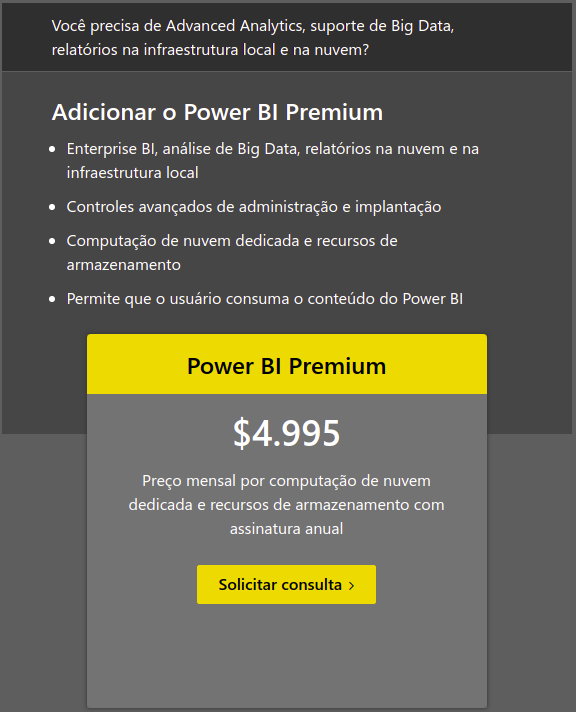
\includegraphics[scale=0.40]{./figures/cap1/powerbi.png}
	\caption{Preço do Power BI Premium}
\end{figure}

\subsection{Qlikview}

O Qlikview é um software desenvolvido pela Qlik, que tem focado os esforços no desenvolvimento do Qlik Sense, que começou como um produto paralelo e agora é o principal. Então, o suporte ao Qlikview está entrando no fim e nem é mais possível consultar os preços dele no site da Qlik. 

Apesar disso, o Qlikview é uma boa ferramenta, oferece um bom conjunto de funções para analisar e apresentar os dados. O Qlik Sense é a evolução dele, com muito mais recursos.

%https://primaconsulting.co.uk/news/2018/3/26/qlikview-vs-qliksense
\subsection{Tableau}

Tableau é uma solução que fornece funcionalidades clique-e-arraste para ajustar dados, criar painéis e visualizações. Existem três produtos dentro dele, o Tableau Desktop, Server e o Online. O preço entre eles varia de \$12,00 até \$70,00 por mês, por licença, podendo ajustar anualmente. É uma das ferramentas mais simples e completas do mercado, exigindo pouco conhecimento do analista por ser clique-e-arraste, por outro lado isso torna um pouco mais difícil o desenvolvimento de análises mais detalhadas.

De modo geral, as principais ferramentas disponíveis são muito similares entre si, todas são competentes, fornecem ótimas funcionalidades, possuem um bom suporte e custam um valor razoavelmente alto, principalmente com o câmbio desfavorecendo o Real. Porém, as ferramentas proprietárias não são as únicas, e para o desenvolvimento do Painel do Centro de Inteligência o Python foi escolhido.



%https://www.betterbuys.com/bi/tableau-pricing/


